\renewcommand{\TheTitle}{Novel MC TRT Method: Vectorizable Variance Reduction for Energy Spectra}
\renewcommand{\TheAuthors}{Joanna Piper Morgan,
  Alex Long,
  Kendra Long, 
  and Kyle E. Niemeyer}
  
\renewcommand{\TheAddress}{
    \textit{Transactions of the American Nuclear Society} \\
    Vol. 126, 318–320, 2022. \\
    \doi{10.13182/T126-38066}
}

\chapter{\TheTitle}
\label{chapter:trt_paper}

\AppendixPaperHeader{\TheTitle}{\TheAuthors}{\TheAddress}

%%%%%%%%%%%%%%%%%%%%%%%%%%%%%%%%%%%%%%%%%%%%%%%%%%%%%%%%%%%%%%%%%%%%%%%%%%%%%%%%
\section{Introduction}
Several production-scale multigroup Thermal Radiation Transport (TRT) codes use the Monte Carlo method as their primary solution technique.
One such example is \textit{Jayenne} from Los Alamos National Lab, which samples a single energy group for a particle then transports it \cite{Thompson_2021}. 
In this work we created a novel TRT variance-reduction method to better resolve the energy spectra with large group structures and fewer particles, with a goal to decrease computational time at a given fidelity of solution in the energy spectra.

\section{TRT Equations}

The explicit TRT equations discretized in frequency using a multigroup approximation, and in zero-dimensional space, are \cite{Pomraning1973}
\begin{equation}
    \frac{1}{c}\frac{\partial I_g(t)}{\partial t} + \sigma_{a,g}(T)I_{g}(t) = x_{g}(T)B_{g}(T)
\end{equation}
%
\begin{equation}
    c_{v}\frac{dE}{dt} = \sum_{0}^{G}{\sigma_{g}(T)I_{g}(t) - x_{g}(T)B_{g}(T)}
\end{equation}
for time $t>0$ and the number of groups $G \geq 1$, where $I_{g}(T)$ is the specific intensity in a given group $g$, $c$ is the speed of light, $\sigma_{a,g}(T)$ is the absorption opacity in a given group g, $B_{g}(T)$ is Planck's function for group $g$, $c_v$ is the specific heat of the material (which is assumed constant), and $x_{g}(T)$ is the Planck-weighted opacity for group $g$.

Note that we discretize the material equation in time using a forward Euler scheme \cite{mc2018}:
\begin{equation}
    T_{n+1} = T_{n} + \frac{\Delta t}{c_{v} \rho}\frac{dE_{n}}{dt} \;,
\end{equation}
where $n$ is the time index and $\rho$ is the material density. 
This means error is proportional to $\mathcal{O}(\Delta t)$.
%%%%%%%%%%%%%%%%%%%%%%%%%%%%%%%%%%%%%%%%%%%%%%%%%%%%%%%%%%%%%%%%%%%%%%%%%%%%%%%%
\section{Flocking Particles}
We propose a method in which a single pseudo-particle carries a vector of energy weights, representing particles across all energy groups in a given simulation.
This could be thought of as a ``flock'' of particles all moving together through space, angle, and time. 
We implement continuous energy deposition so a distance to event is found by comparing the distance to a spatial cell boundary and a distance associated with the time left in a step (effectively the temporal cell boundary) and selecting the minimum between the two.
We are considering several ways to implement physical scattering, which is not currently implemented in this work. 
A scheme with explicit Euler does not introduce ``effective scattering'' and physical scattering is generally much smaller than absorption opacity.

%Scattering is not currently implemented, as physical scattering is much smaller than effective scattering for most simulations neglecting however and/or giving it special treatment in the future is totally.
%add more info about combing to this section

We also required this method to be time dependant by using a particle census to move particles between time steps.
A known, desired number of particles is used to find the census population (particles brought forward from the last time step) and emission population (particles produced by material emission within a time step) governed by their ratio of total energy.
If the population of the census is larger than its allocation, then we use Russian Roulette for population control (based on Legrady et al.~\cite{Legrady2020}).
This addresses the unbounded particle growth that happens when implementing continuous energy methods.

A Roulette normally does not conserve either total energy or total group energy for a finite number of particles; our method requires both. 
This is due to our desire to conserve spectral shape to hopefully lead to further variance reduction.
This requirement means that if the energy weight for a given group across all particles was computed, it would be the same before and after the Roulette, as well as total energy of all particles.
Figure 1~\ref{fig:roulette} shows the population Roulette, where a vector of energy weights is accumulated for each Rouletted particle in each group. That accumulation vector is then divided by the number of particles remaining at the end of the Roulette. And finally this per particle accumulation vector of energy weights is added to the energy of the still living census particles, group by group.
Histories will only terminate when met with the end of the problem or the Roulette.

\begin{figure}
    \begin{center}
        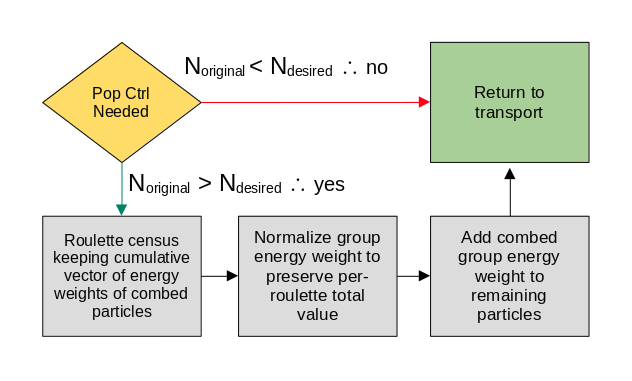
\includegraphics[width=.75\textwidth]{appendix/trt_figs/flow_chart.png}
        \caption{Flowchart of the Russian Roulette population control process as implemented in our method.}
        \label{fig:roulette}
    \end{center}
\end{figure}

After a distance to event is sampled, the energy weights in \textbf{all} groups must be attenuated, requiring the computation of an exponential function, and the manipulation of energy weights in \textbf{all} groups.
This is done independently as if it were a normal particle in that energy group by
\begin{equation}
    w_g^{n+1} = w_g^n e^{-\sigma_g  d} \;,
\end{equation}
where $w$ is the energy weight of a particle, $n$ is the time index, $g$ is the group number, and $d$ is the distance to event (same distance across all groups).

Consider a 200-group problem using our novel technique: instead of computing a single exponential attenuation as in the single-group MC scheme, we must repeat this exponential calculation 200 times (once for each frequency group in the problem).
Thus for \textit{one} pseudo-particle's history, in \textit{one} time step, the number of exponentials required is now proportional to the number of groups, hindering effective performance gains.

However, there is still hope.
The attenuation calculation involves applying the same operation to multiple discrete pieces of data; said another way, the attenuation calculation is an example of single instruction/multiple data (SIMD) processing.
SIMD hardware (a type of vector-processing unit) is widely deployed, and can be found in production x86 CPUs with AVX instructions as well as machines purpose-built to operate on vectors. 
It is also relatively easy to enable through the use of compiler flags on modern C++ compilers \cite{OpenMP2018}. 
As a result, this method will be able to use accelerators that already exist and commonly remain idle, to speed up our novel method and dampen the hit to performance.

% add difference to the other work
The method presented here is similar to, though distinct from, a method described by McKinley, Brooks, and Szoke~\cite{McKinley2003}.
They apply a vector-of-weights approach to the Symbolic Implicit Monte Carlo (SIMC) algorithm, while this method is applied directly to a time-explicit discretization of the TRT equations.
We also investigate this method for specific use on vector hardware.

%%%%%%%%%%%%%%%%%%%%%%%%%%%%%%%%%%%%%%%%%%%%%%%%%%%%%%%%%%%%%%%%%%%%%%%%%%%%%%%%
\section{Results and Discussion}
We developed a test code in C++ to examine this method's performance, first as a time-dependent zero spatial dimension problem, then as a time-dependent single spatial dimension problem. 
For both we ran gray and multigroup test cases and compared results to analytical solutions (if available) as well as the \textit{Jayenne} Implicit Monte Carlo code from Los Alamos National Lab.

\subsection{Zero-dimensional problem}

The zero-dimensional test is a simple time-dependent equilibration problem. We compared a gray case to both the analytical Mosher \cite{Mosher2006} solution as well as solutions from Jayenne. Then, we performed simulations with up to 200 energy groups in Jayenne, examining both time to equilibration and the spectrum of the results.

Table~\ref{tabel:0d_error} shows that to get roughly the same fidelity of solution our novel method required the simulation of only \num{1e4} particles, while the production code required \num{1e6} particles.
These were computed against a benchmark solution from the production code of \num{5e6} particles.
With these results we felt confident to move our novel method into one dimension.

\begin{table}
    \caption{L2 norms between Jayenne and Flocking for the zero-dimensional solution. Flocking at \num{1e4} particles is as accurate as Jayenne at \num{1e6}.}
    \centering
    \begin{tabular}{@{}llll@{}}
        \toprule
         Time Step & Jayenne (\num[print-unity-mantissa=false]{e4}) & Jayenne (\num[print-unity-mantissa=false]{e6}) & Flocking (\num[print-unity-mantissa=false]{e4}) \\
         \midrule
         1000 & \num{1.03e-1} & \num{4.60e-3} & \num{3.66e-3} \\
         2000 & \num{7.59e-2} & \num{4.53e-3} & \num{3.83e-3} \\
         \bottomrule
    \end{tabular}
    \label{tabel:0d_error}
\end{table}


\subsection{One-dimensional problem}

To compare the results of our testbed with those from Jayenne, we employ a Marshak wave test, again starting from the gray case, then moving to multigroup with up to 200 groups.
The test case is a \SI{1}{\centi\meter} long slab of iron ($c_v$ = \SI{0.1}{\giga\joule\per\gram\per\kilo\eV}, $\rho$ = \SI{1}{\gram\per\cm^3}), where the material and radiation temperatures are initially at equilibrium at \SI{1e-6}{\kilo\eV}.
The left boundary is an infinite plane wall source, with temperature \SI{3}{\kilo\eV} and the right boundary is a vacuum.
We used a time step of $\Delta t$ =  \SI{e-12}{\s} and a mesh width of $\Delta x$ = \SI{0.005}{\cm}
As time goes forward we expect a temperature wave to propagate through the material from left to right.
As time goes to infinity we expect the solution to come to equilibrium.

After confirming that the temperature profiles over time matched both our expectations and solutions from Jayenne, we moved to examine their spectra in specific mesh cells at specific time steps. 
Figure~\ref{fig:10kvar} shows the spectrum produced by either code at ten-thousand particles compared to a benchmark solution of the production code ran with 5 million particles. 
The spectral solution from Jayenne is very noisy (lots of jagged peaks) while the spectrum produced by our novel method is smooth and accurate compared to the benchmark solution at this low particle count.
This demonstrates that the variance reduction works.

However, a slight deviation of the spectral shape near the peak is observed.
We believe this stems from the use of spatial tilt for source position sampling in Jayenne that has not yet been implemented in our test-bed code.
When implemented we expect this discrepancy to disappear and we will be able to use a traditional Figure of Merit comparison to fully demonstrate the novel method's variance reduction abilities.

\begin{figure}
    \begin{center}
        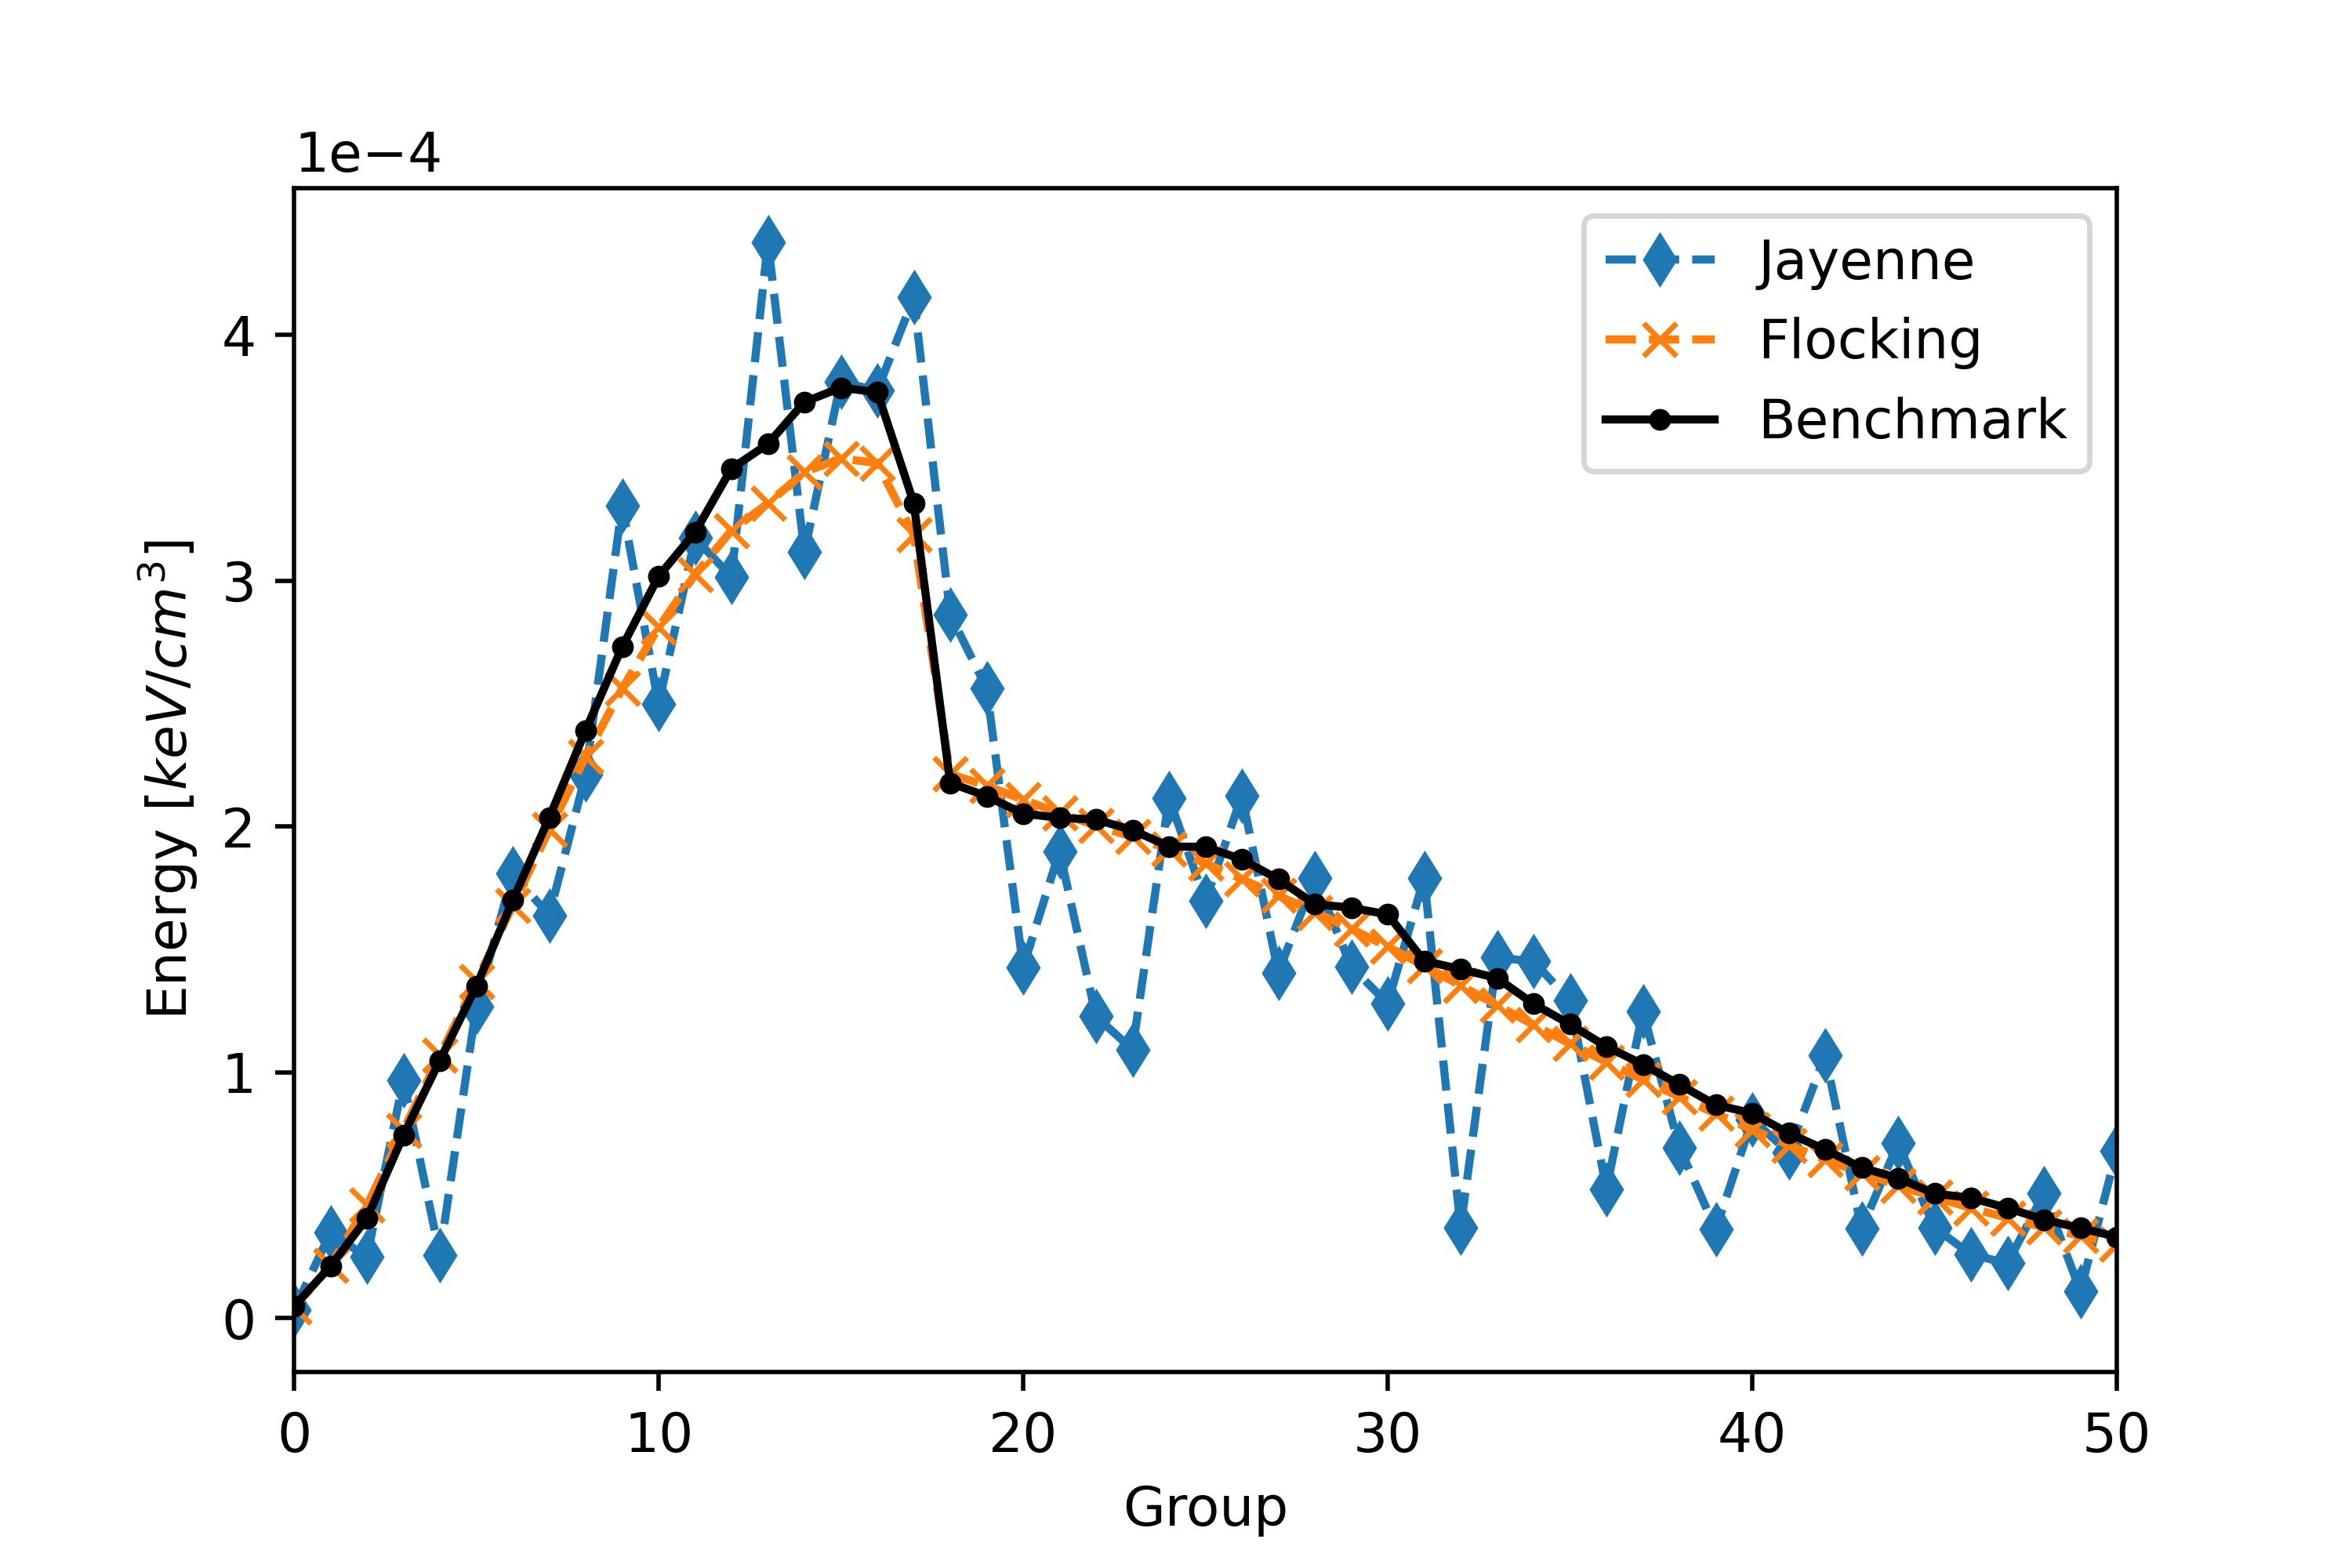
\includegraphics[width=\textwidth]{appendix/trt_figs/spectra_report.png}
        \caption{Energy spectra from a single cell at a single time step produced with \num{1e4} particles to show the high-variance solution produced from Jayenne, and the low-variance solution produced by our novel method. They are plotted against a benchmark solution from Jayenne computed with \num{5e6} particles.}
        \label{fig:10kvar}
    \end{center}
\end{figure}

We must also consider run times. 
Table~\ref{table:flockvec} confirms that this method is vectorizable, and will be able to take advantage of the specialized vector processing components of modern CPUs.
It also shows that enabling vectorization has a huge impact on run time for this method; cutting runtime for a fully optimized executable (using the Intel icpc compiler flag \texttt{-Ofast}) in half when they are turned on (using a SIMD reduction flag above the attenuation loop).

To confirm that this method will result in an overall performance increase when considering the energy spectra, we raced the production code against the novel method at various particle counts and examined their spectra. 
Table~\ref{table:jayandflock} shows that the novel method does take slightly longer. However, if a well resolved spectrum is the goal of the computation then we have effectively reduced the computational time as fewer particles are required to get a well defined solution. While direct comparisons to production codes can be fraught, we feel this demonstrates that if this method is implemented in Jayenne the figure of merit will increase.

\begin{table}
\caption{Run-times of the 1D novel method test bed under various compiler flag conditions. Simulations run on a single node of Intel Skylake Gold processors.}
\begin{center}
    \begin{tabular}{@{}lll@{}}
         \toprule
         Optimized? & Vectorized? & Runtime [s]\\
         \midrule
         no & no & 1855.2\\
         yes & no & 353.2\\
         yes & yes & 184.7\\
         \bottomrule
    \end{tabular}
    \label{table:flockvec}
\end{center}
\end{table}

\begin{table}[]
\caption{Comparing the run-times of the 1D test case between Jayenne and flocking test bed.}
    \begin{center}
    \begin{tabular}{@{}lll@{}}
         \toprule
          Method & \# particles & Runtime [s] \\
         \midrule
         Jayenne & \num{1e4} & 70.97 \\
         Jayenne & \num{1e6} & 3005.50 \\
         flocking & \num{1e4} & 92.0 \\
         flocking & \num{1e6} & 3775.12  \\
         \bottomrule
    \end{tabular}
    \label{table:jayandflock}
    \end{center}
\end{table}

%%%%%%%%%%%%%%%%%%%%%%%%%%%%%%%%%%%%%%%%%%%%%%%%%%%%%%%%%%%%%%%%%%%%%%%%%%%%%%%%
\section{Conclusions}

We have successfully demonstrated a novel variance reduction technique for the energy spectra for Monte Carlo Thermal Radiation Transport. Continued work is required before the method is stable enough to implement on production codes. Specifically we need to implement physical scattering, source tilting \cite{Wollaber2016}, and post-collisions group splitting (to prevent highly unlikely interactions across various energy regimes in optically thin material) in the testbed.

%%%%%%%%%%%%%%%%%%%%%%%%%%%%%%%%%%%%%%%%%%%%%%%%%%%%%%%%%%%%%%%%%%%%%%%%%%%%%%%%

\section*{Acknowledgments}
Release number: LA-UR-22-20908.

This work was supported by the Center for Exascale Monte-Carlo Neutron Transport (CEMeNT) a PSAAP-III project funded by the Department of Energy, grant number: DE-NA003967.


